\documentclass[tikz,border=4pt]{standalone}
\usepackage{amsmath,amssymb}
\usetikzlibrary{arrows.meta,positioning,calc}
\hyphenpenalty=10000
\exhyphenpenalty=10000

\begin{document}
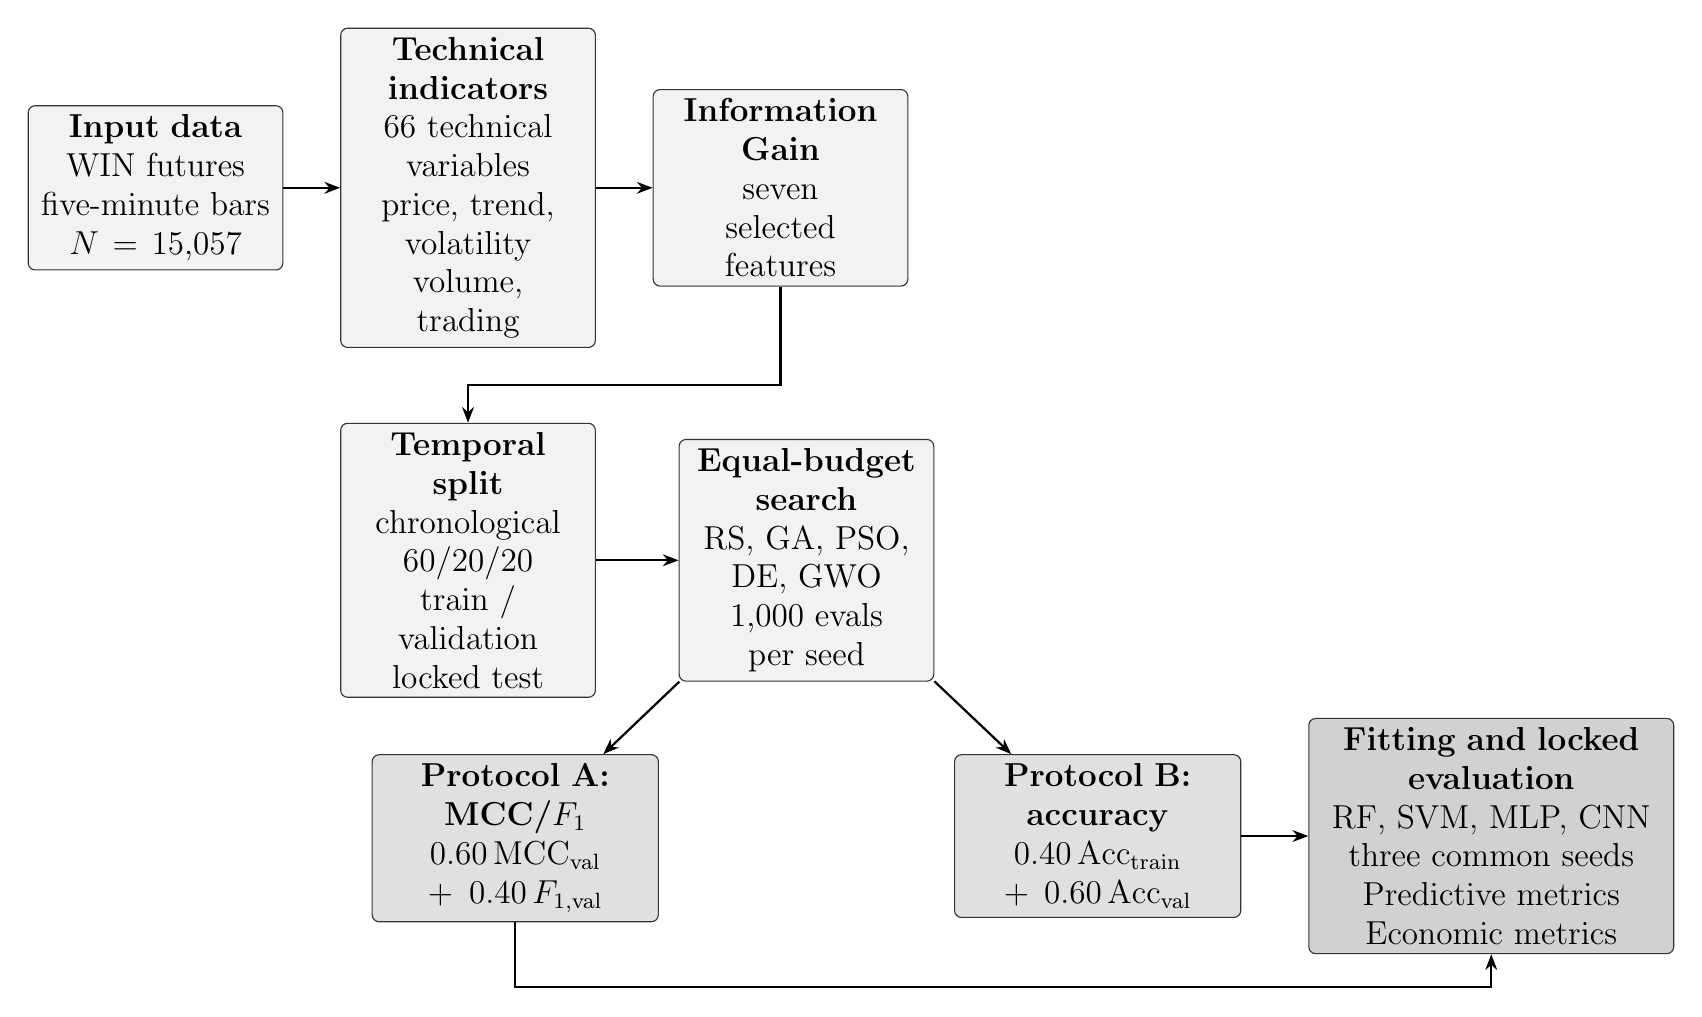
\begin{tikzpicture}[
  node distance=0.82cm and 0.72cm,
  every node/.style={draw=black!80,rounded corners=2.5pt,align=center,minimum height=0.88cm,text width=3.0cm,font=\large},
  process/.style={fill=black!5}, protocol/.style={fill=black!12,text width=3.4cm},
  outcome/.style={fill=black!18,text width=4.4cm}, arrow/.style={-{Stealth[length=2.0mm]},thick}
]
  \node[process] (data) {\textbf{Input data}\\WIN futures\\five-minute bars\\$N=15{,}057$};
  \node[process, right=of data] (indicators) {\textbf{Technical}\\\textbf{indicators}\\66 technical\\variables\\price, trend,\\volatility\\volume,\\trading};
  \node[process, right=of indicators] (selection) {\textbf{Information}\\\textbf{Gain}\\seven\\selected\\features};
  \node[process, below=0.95cm of indicators] (split) {\textbf{Temporal split}\\chronological\\60/20/20\\train /\\validation\\locked test};
  \node[process, right=1.05cm of split] (search) {\textbf{Equal-budget}\\\textbf{search}\\RS, GA, PSO,\\DE, GWO\\1,000 evals\\per seed};
  \node[protocol, below left=0.92cm and 0.25cm of search] (mcc) {\textbf{Protocol A:}\\\textbf{MCC/$F_1$}\\$0.60\,\mathrm{MCC}_{\mathrm{val}}$\\$+\;0.40\,F_{1,\mathrm{val}}$};
  \node[protocol, below right=0.92cm and 0.25cm of search] (accuracy) {\textbf{Protocol B:}\\\textbf{accuracy}\\$0.40\,\mathrm{Acc}_{\mathrm{train}}$\\$+\;0.60\,\mathrm{Acc}_{\mathrm{val}}$};
  \node[outcome, right=0.85cm of accuracy] (test) {\textbf{Fitting and locked}\\\textbf{evaluation}\\RF, SVM, MLP, CNN\\three common seeds\\Predictive metrics\\Economic metrics};
  \draw[arrow] (data) -- (indicators);
  \draw[arrow] (indicators) -- (selection);
  \coordinate (splitroute) at ($(split.north)+(0,0.48cm)$);
  \draw[arrow] (selection.south) |- (splitroute) -- (split.north);
  \draw[arrow] (split.east) -- (search.west);
  \draw[arrow] (search) -- (mcc);
  \draw[arrow] (search) -- (accuracy);
  \coordinate (mccroute) at ($(test.south)+(0,-0.42cm)$);
  \draw[arrow] (mcc.south) |- (mccroute) -- (test.south);
  \draw[arrow] (accuracy.east) -- (test.west);
\end{tikzpicture}
\end{document}
